\documentclass[conference]{IEEEtran}

\usepackage{graphicx}
\usepackage{xcolor}
\usepackage{interval}
\usepackage{amsmath, amssymb}
\usepackage{cuted, tcolorbox}
\usepackage{tikz}
\usepackage[ruled,vlined]{algorithm2e}
\usepackage{algpseudocode}

\usepackage{subcaption}

\usepackage{amssymb}% http://ctan.org/pkg/amssymb
\usepackage{pifont}% http://ctan.org/pkg/pifont
\newcommand{\cmark}{\ding{51}}%
\newcommand{\xmark}{\ding{55}}%

\usepackage[hyphens]{url}
\usepackage[normalem]{ulem}

\makeatletter
\newcommand{\printfnsymbol}[1]{%
  \textsuperscript{\@fnsymbol{#1}}%
}
\makeatother

\newcommand{\RH}[1]{\textcolor{blue}{#1}}
\newcommand{\JS}[1]{\textcolor{red}{#1}}
\newcommand{\TODO}[1]{\textcolor{red}{TODO: #1}}
\newcommand{\HY}[1]{\textcolor{brown}{#1}}

% blue comment
\newcommand\mycommfont[1]{\footnotesize\ttfamily\textcolor{blue}{#1}}
\SetCommentSty{mycommfont}
% blue triangle
\SetKwComment{Comment}{\color{blue} $\triangleright$\ }{}

\begin{document}

\title{VRF-based mining}

% \author{
%     \IEEEauthorblockN{
%         Runchao Han\IEEEauthorrefmark{1}\IEEEauthorrefmark{2}, 
%         Haoyu Lin,
%         Jiangshan Yu\IEEEauthorrefmark{1}
%     }
%     \IEEEauthorblockA{
%         \IEEEauthorrefmark{1}Monash University\\
%         \IEEEauthorrefmark{2}CSIRO-Data61
%     }
% }

\maketitle

\begin{abstract}
  In this paper, we introduce VRF-based mining, a simple and effective way of making pooled mining impossible.
  Instead of using hash functions, VRF-based mining uses Verifiable Random Functions (VRFs) for Proof-of-work (PoW)-based consensus.
  As VRF binds the authorship with hashes, a pool operator should reveal his private key to outsource the mining process to miners, and miners can anonymously steal cryptocurrency in the pool operator's wallet.
  
  We informally revisit the definition of non-outsourceability in existing research, and show VRF-based mining achieves stronger non-outsourceability than all existing proposals.
  We also discuss several considerations on instantiating VRFs for VRF-based mining.
  In addition, we experimentally show that VRF-based mining is easy to implement, and introduces little overhead compared to hash-based mining.
  Moreover, we discuss why partial outsourcing in VRF-based mining is unprofitable, and how to make it even more unprofitable.
\end{abstract}

\section{Introduction}
\label{sec:intro}

Bitcoin~\cite{nakamoto2008bitcoin} started the era of cryptocurrency.
Bitcoin's main novelty is Nakamoto consensus - the first consensus protocol that can work in permissionless settings.
% blockchain
In Nakamoto consensus, each participant maintains its own ledger, and the ledger is usually called blockchain.
A blockchain is formed as a chain of blocks, and each block contains a batch of transactions.
Blockchain is designed to be append-only, and its integrity is protected by digital signatures.
% proof of work
Participants keep appending blocks to the blockchain.
To append a block, a participant should first solve a Proof-of-Work (PoW)~\cite{dwork1992pricing} puzzle - a probabilistic and moderately hard computation puzzle.
Once solving the puzzle, the participant will append his block to the blockchain, and get some cryptocurrency as reward.
By adaptively adjusting the difficulty of PoW puzzles, Nakamoto consensus can stabilise the speed of generating blocks.
Participants of Nakamoto consensus are also known as miners, the process of solving PoW puzzles is known as mining, and the computation power used for mining is known as mining power.

% why pooled mining
Today, mining pools dominate the mining power of most blockchains using Nakamoto consensus.
Mining pool is a kind of service that gathers mining power from solo miners and rewards solo miners in a more fine-grained way.
More specifically, a single blockchain may consist of numerous miners, and each miner may have a low chance to mine the next block, leading to unstable mining reward.
A mining pool allows miners to mine on blockchain in the name of the pool operator, and the pool operator distributes the mining reward to solo miners according to their contributed mining power.
In this way, a miner can get reward more stably by joining a mining pool.

% Problems of having mining pools
However, mining pools lead to centralisation of mining power, which contradicts the design objective of Bitcoin - the decentralisation.
% problem of centralisation
Centralisation of mining power can be harmful for the security of Nakamoto consensus.
A mining pool with sufficient mining power can perform numerous types of attacks to break the consensus, such as selfish mining attacks~\cite{eyal2018majority} and 51\% attacks~\cite{nakamoto2008bitcoin}.
Even top mining pools are not big enough, multiple mining pools can even collude to launch attacks.
In addition, mining pools can decide which transactions to include in order to censor the blockchain.
% to date...
To date (01/12/2019), four largest mining pools control more than 51\% Bitcoin mining power, which can be a lurking threat of Bitcoin.




\textbf{Our contributions.}
In this work, we put forward a novel idea of combining VRF and mining in PoW to eliminate the intentionality of pooled mining, and to conquer the centralisation of mining power. We call our construction \textbf{VRF-based mining}.

\TODO{We should make the contribution part more sophisticated here. At least we have the following contributions:
Main: We propose the VRF-based mining that makes pooled mining impossible. In particular, we
1. Propose the detailed construction of VRF-based mining, which can be a drop-in replacement of existing hash-based mining (we already have)
2. We rethink the desired properties of mining that can make pooled mining difficult while remaining secure (Runchao will do this later)
3. We justify the security and non-outsourcability of VRF-based mining against existing attacks and vulnerabilities (Runchao)
4. We analyse cons of having no mining pool and possible solutions (Haoyu)
5. We discuss how to discourage pooled staking using VRF (Haoyu)
}

\textbf{Paper organisation.}
% \TODO{we should have a paragraph describing the organisation of this paper. See the paper ``New Techniques for Efficient Trapdoor Functions and Applications''}
We revisit the concepts of mining, the standard definitions and the properties of VRF and EC-VRF in Section~\ref{sec:preliminaries}.
We give our construction of VRF-based mining in Section~\ref{sec:construction} and \ref{sec:instantiation},
and then analyse its non-outsourceability in Section~\ref{sec:non_outsourceability}.
Finally, we discuss the \TODO{XXX} in Section~\ref{sec:problems-and-solutions},
and the related work in Section~\ref{sec:related}.

\section{Preliminaries}

\subsection{Cryptocurrency mining}

In cryptocurrency mining, miners search for the solution to a computational puzzle.
Specifically, the puzzle is to find a (partial) pre-image for a cryptographic hash function, of which output is less than a target value begining with several consecutive zero bits.
The hash function maps a list of transaction, the hash of the previous block, a timestamp, an nonce and other information, to a result value.
As the hash result is unpredictable and unformly distributed, the probability of the hash result lies among the desired interval is inversely proportional to the number of leading zero.

The more computation power the miner possesses, the more rounds of hash he can run during a time unit, and the more likely he can find the solution. The first miner who finds the solution and anounces it, wins the competition and gets rewarded.

\subsection{Verifiable random functions}

Verifiable Random Function (VRF)~\cite{micali1999verifiable} is a public-key version of cryptographic hash function.
It involves a pair of a secret key and a public key.
Only the owner of the secret key can compute the hash, while anyone having the public key can verify the hash.
Formally, a VRF consists of four algorithms: $\mathsf{VRFKeyGen}$, $\mathsf{VRFHash}$, $\mathsf{VRFProve}$ and $\mathsf{VRFVerify}$.

\begin{itemize}
    \item $(sk, pk) \gets \mathsf{VRFKeyGen}(1^{\lambda})$: on input a security parameter $1^{\lambda}$, outputs the secret/public key pair $(sk, pk)$.
    \item $\beta \gets \mathsf{VRFHash}(sk, \alpha)$: on input $sk$ and an arbitrary-length string $\alpha$, outputs a fixed-length hash $\beta$.
    \item $\pi \gets \mathsf{VRFProve}(sk, \alpha)$: on input $sk$ and $\alpha$, outputs the proof $\pi$ for $\beta$.
    \item $\{0, 1\} \gets \mathsf{VRFVerify}(pk, \alpha, \beta, \pi)$: on input $pk$, $\alpha$, $\beta$, $\pi$, outputs the verification result 0 or 1.
\end{itemize}


\section{VRF-based mining}

\subsection{Our construction}

We replace hash function in mining by VRF, and thus construct VRF-based mining.

To rule out pooled mining, we combine VRF with digital signature scheme.
As the digital signature scheme use in cryptocurrency are based on Elliptic curve, we construct Elliptic curve based VRF for our VRF-based mining.
The standardised construction is put in the appendix~\ref{vrf_standardised_construction}.

% The desired properties of a well-designed hash function includes uniformity, deterministic, unpredictability and verifiability.
% As shown in appendix~\ref{vrf_standardised_construction}, ...
% Therefore, VRF fits in here.

In the case of solo mining, our sheme works as follows.

\TODO{change format to algorithm2e}
% https://www.overleaf.com/learn/latex/algorithms
\begin{enumerate}
    \item The solo miner runs $\mathsf{VRFKeyGen}(1^{\lambda})$ to generate a secret key and public key pair $(sk, pk)$.
    \item The miner queries the the full node it runs, and build a block template, including a coinbase transaction paying to him, for example, to his \texttt{scriptPubKey}.
    \item The miner alters the nonce in the block header.
    \item The miner takes the block header as $\alpha$, and runs $\mathsf{VRFHash}(sk, \alpha)$ to get $\beta$. If $\beta$ meets the difficulty requirement, a block is found; otherwise, the miner changes the nonce and runs $\mathsf{VRFHash}(sk, \alpha)$ again.
    \item The miner runs $\mathsf{VRFProve}(sk, \alpha)$ to generate a proof $\pi$.
    \item The miner then submit the $pk$, $\beta$, and the proof $\pi$ to the node.
    \item The node then check:
        \begin{enumerate}
            \item if $\beta$ meets the difficulty requirement;
            \item if $\mathsf{VRFVerify}(pk, \alpha, \beta, \pi)$ result is valid;
            \item whether the \texttt{scriptPubKey} in the coinbase transaction corresponds to $pk$.
        \end{enumerate}
        If all results are valid, a new block is mined, and the coinbase reward is paid to the miner.
    \item $pk$, $\beta$ and $\pi$ should also be recorded in the block header, so that, when the block is propogated to other nodes, they can easily validate it via $\mathsf{VRFVerify}(pk, \alpha, \beta, \pi)$.
\end{enumerate}

\subsection{Why pooled mining cannot work in our scheme}

% need private key
As shown in appendix~\ref{vrf_standardised_construction}, both $\mathsf{VRFHash}$ and $\mathsf{VRFProve}$ take secret key $sk$ as input.
That is to say, if a pool operator would like to provide pooled mining service and let miners participate, he will need to provide miners with his secret key.

% none would like to provide private key
However, none rational pool operator will tend to give out his secret key, as revealing his secret key give others the opportunity to redeem his balance or forge his identity.

Therefore, following our construction, we eliminate the intentionality of pooled mining and can reduce the centralisation of mining power significanlty.

\section{Non-outsourceability analysis}
\label{sec:non_outsourceability}

% \cite{miller2015nonoutsourceable} first formally defines cryptocurrency mining as scratch-off puzzles. \TODO{describe}

% \begin{description}
%     \item[Correctness] Any valid hash can be verified.
%     \item[Feasibility] Mining is computationally feasible.
%     \item[Parallelisability] The mining process can be parallelised.
%     \item[$\mu$-Imcompressibility] The adversary cannot accelerate the mining process using pre-generated pairs of nonces and hashes, by at most a factor $\mu$ ($\mu \geq 1$). If $\mu = 1$, $\mathsf{Work}$ is the optimal way to mine.
%     \item[Non-transferability] Given a block template, the adversary cannot accelerate the mining process using other valid hashes on this block template.
% \end{description}

\subsection{Revised definitions}

Miller et al. \cite{miller2015nonoutsourceable} first formalises cryptocurrency mining as non-outsourceable scratch-off puzzles, and formally defines non-outsourceability.
In particular, they define two levels of non-outsourceability, namely \textbf{Weak Non-outsourceability} and \textbf{Strong Non-outsourceability}.

\begin{description}
    \item[Weak Non-outsourcability] If the pool operator outsources the mining process, miners can always steal the reward of mining.
    \item[Strong Non-outsourcability] In addition to the Weak Non-outsourcability, the pool operator cannot link the stolen mining reward with the miner who steals it.
\end{description}

Basically, \textbf{Weak Non-outsourceability} defines the punishment of outsourcing, while \textbf{Strong Non-outsourceability} covers both the punishment and the anonymity of malicious miners.
We call the property defining the punishment of outsourcing \textbf{Punish-mining-reward}.
The anonymity of malicious miners defined in~\cite{miller2015nonoutsourceable} is equivalent to \textbf{Transaction Unlinkability}~\cite{van2013cryptonote}: given two arbitrary transactions, distinguishing whether they have the same output address requires knowing the private keys holding their outputs.
To steal the mining reward, the miner should create a transaction, of which the input is the mining reward and the output is his owned address.
Identifying who steals the mining reward is equivalent to finding out who holds the output address, which can be further reduced to \textbf{Transaction Unlinkability}.


\subsection{Punish-secret-key-leakage}

% SK-non-outsourceability
We introduce \textbf{Punish-secret-key-leakage}, a new property of punishment on outsourcing that achieves stronger non-outsourceability than \textbf{Punish-mining-reward}.
A cryptocurrency mining protocol achieves \textbf{Punish-secret-key-leakage} in the following sense: the pool operator should reveal 1) the block template and 2) the private key receiving the coinbase transaction, so that miners can mine in the name of the pool operator.

% stronger than weak non-out
In a cryptocurrency mining protocol with \textbf{Punish-secret-key-leakage}, the pool operator should reveal his private key to miners, which gives miners opportunity to steal all cryptocurrency in the pool operator's wallet.
This indicates that, in terms of the punishment of outsourcing, \textbf{Punish-secret-key-leakage} is stronger than \textbf{Punish-mining-reward}, where miners can only steal the mining reward part.






\subsection{Non-outsourceability of VRF-based mining}

VRF-based mining achieves both \textbf{Punish-secret-key-leakage} and \textbf{Transaction Unlinkability}.
In VRF-based mining, the pool operator outsources mining requires revealing his private key to miners, which leads to \textbf{Punish-secret-key-leakage}.
Similar with the construction achieving \textbf{Strong Non-outsourceability} in~\cite{miller2015nonoutsourceable}, VRF-based mining achieves \textbf{Transaction Unlinkability} by allowing a malicious miner to use a freshly generated address to steal cryptocurrency.
To receive the stolen cryptocurrency of the pool operator, the malicious miner can create a new address, and construct a transaction of which the stolen cryptocurrency directs to this address.
As this new address has no historical transactions, linking the transaction stealing cryptocurrency with other transactions can be impossible.
Then the malicious miner can then spend his stolen cryptocurrency anonymously using numerous techniques, such as mixing services~\cite{maxwell2013coinjoin}\cite{bonneau2014mixcoin}\cite{ruffing2014coinshuffle}\cite{heilman2017tumblebit} and stealth addresses~\cite{van2013cryptonote}.



\section{Instantiating VRF}

In order to implement VRF-based mining, one needs to first instantiate the VRF.
VRF has four configurable components, namely the elliptic curve and three hash functions $H_{1}(\cdot)$, $H_{2}(\cdot)$ and $H_{2}(\cdot)$.
$H_{1}(\cdot)$ maps an arbitrary-length string into an elliptic curve element;
$H_{2}(\cdot)$ maps an elliptic curve element into a fixed-length string; and
$H_{3}(\cdot)$ maps an arbitrary-length string into a fixed-length string.
In this section, we discuss considerations on choosing these four components for VRF-based mining.





\subsection{Elliptic curve}

As neither blockchains and VRF limits the choice of elliptic curves, any elliptic curve can be adapted.
Among prominent elliptic curves, Curve25519~\cite{} can be a promising choice.
Curve25519 supports Ed25519~\cite{}, a fast and secure digital signature algorithm.
In addition, numerous blockchains~\cite{} and projects using VRF~\cite{} adapt Ed25519 as their underlying elliptic curve.




\subsection{$H_{1}(\cdot)$ (hashing a string to an elliptic curve point)}

% indistinguishable
$H_{1}(\cdot)$ is a hash-to-curve function, which should prevent distinguishing behaviours: adversaries cannot learn any pattern of the input from its hash.
% deterministic
In addition, the hash-to-curve function used in VRF should be deterministic, otherwise the hash will be unreproducible.

A standardisation document~\cite{} specifies several hash-to-curve functions that fit into different elliptic curves and satisfy our requirements: Icart Method~\cite{}, Shallue-Woestijne-Ulas Method~\cite{}, Simplified SWU Method~\cite{} and Elligator2~\cite{}.
Within these hash-to-curve functions, Elligator2 is the recommended one for Curve25519.




\subsection{$H_{2}(\cdot)$ (hashing an elliptic curve point to a string)}

$H_{2}(\cdot)$ hashes an elliptic curve point to a fixed-length string.
It can be divided to two steps: 1) encoding an elliptic curve point to a string, and 2) hashing the string using a normal hash function.
The encoding step can be bidirectional and unencrypted, so can be done simply by converting a big integer to a string.
The hashing step should be cryptographically secure, so can adapt any existing cryptographically secure hash functions.

For ASIC-resistant cryptocurrencies using memory-hard hash functions (e.g., Ethereum~\cite{} and Monero~\cite{}), there are some concerns on choosing hash functions in $H_{2}(\cdot)$.
% VRFHash shoule memory-hard
To make mining memory-hard, $\mathsf{VRFHash}$ should be memory-hard.
% vrfhash steps
$\mathsf{VRFHash}$ of the standardised VRF consists of one $H_{1}(\cdot)$ hashing, one scalar-point multiplication and one $H_{2}(\cdot)$ hashing.
$H_{1}(\cdot)$ and the encoding step in $H_{2}(\cdot)$ can be fast so less possible to become the performance hotspot.
The scalar-point multiplication is slow and computation (rather than memory)-intensive.
% make VRFHash memory hard
The hash function in $H_{2}(\cdot)$ is the only possibility to make $\mathsf{VRFHash}$ memory-hard, and it should be overwhelmingly slower than the scalar-point multiplication, otherwise the scalar-point multiplication will make $\mathsf{VRFHash}$ computation-intensive.
This requirement can be achieved by repetitively executing one or multiple different memory-hard hash functions (such as Ethash~\cite{}, Equihash~\cite{}, and CryptoNight~\cite{}).





\subsection{$H_{3}(\cdot)$ (Normal hash function)}

$H_{3}(\cdot)$ is only used in $\mathsf{VRFProve}$ (proving the authorship of hashes) and $\mathsf{VRFVerify}$ (verifying the authorship of hashes).
The overhead of proving and verification should be minimised, so cryptographically secure hash functions that are designed to be fast (such as Keccak~\cite{} and BLAKE~\cite{}) are suitable for $H_{3}(\cdot)$.
\section{Practicality of VRF-based mining}
\label{sec:practicality}

In this section, we experimentally show that VRF-based mining is easy to implement and introduces little overhead.
Our experiment is twofold.
First, we compare the performance of VRFs with three other hash functions used for cryptocurrency mining, namely SHA256D used in Bitcoin, Scrypt used in Litecoin and CryptoNight used in Monero.
The comparison shows that VRF can be much faster than Ethereum and CryptoNight.
Second, we measure the runtime of each step ($H_1(\cdot)$, point multiplication and $H_2(\cdot)$) of $\mathsf{VRFHash}$.
The result shows that the elliptic curve scalar multiplication dominates $\mathsf{VRFHash}$'s runtime, which can be optimised in the future.

\subsection{Experimental setting}

We implement the standardised EC-VRF in Algorithm~\ref{algo:standard-ecvrf} using Go programming language.
In particular, we use Ed25519~\cite{bernstein2012high} as the underlying elliptic curve, Elligator~\cite{bernstein2013elligator} as $H_1(\cdot)$, SHA-3 as the hash function.
Ed25519, SHA-3 and the encoding of points on Ed25519 are supported by Go's standard library.
We do not apply any optimisation on the EC-VRF implementation.
We use open-source implementations basing on their popularity on \url{https://github.com/} for SHA256D~\footnote{\url{https://github.com/seehuhn/sha256d}}, Scrypt~\footnote{\url{https://github.com/elithrar/simple-scrypt}}, and CryptoNight~\footnote{\url{https://github.com/Equim-chan/cryptonight}}.

All experiments run on a MacBook Pro with a 2.2 GHz Intel Core i7 Processor, a 16 GB DDR4 RAM and 256 SSD storage disk.
For each group of experiment, we run an algorithm for ten times, then take the average data as the experimental results.




\subsection{Comparison between VRF and other mining algorithms}

\begin{figure}[htp]
    \centering
    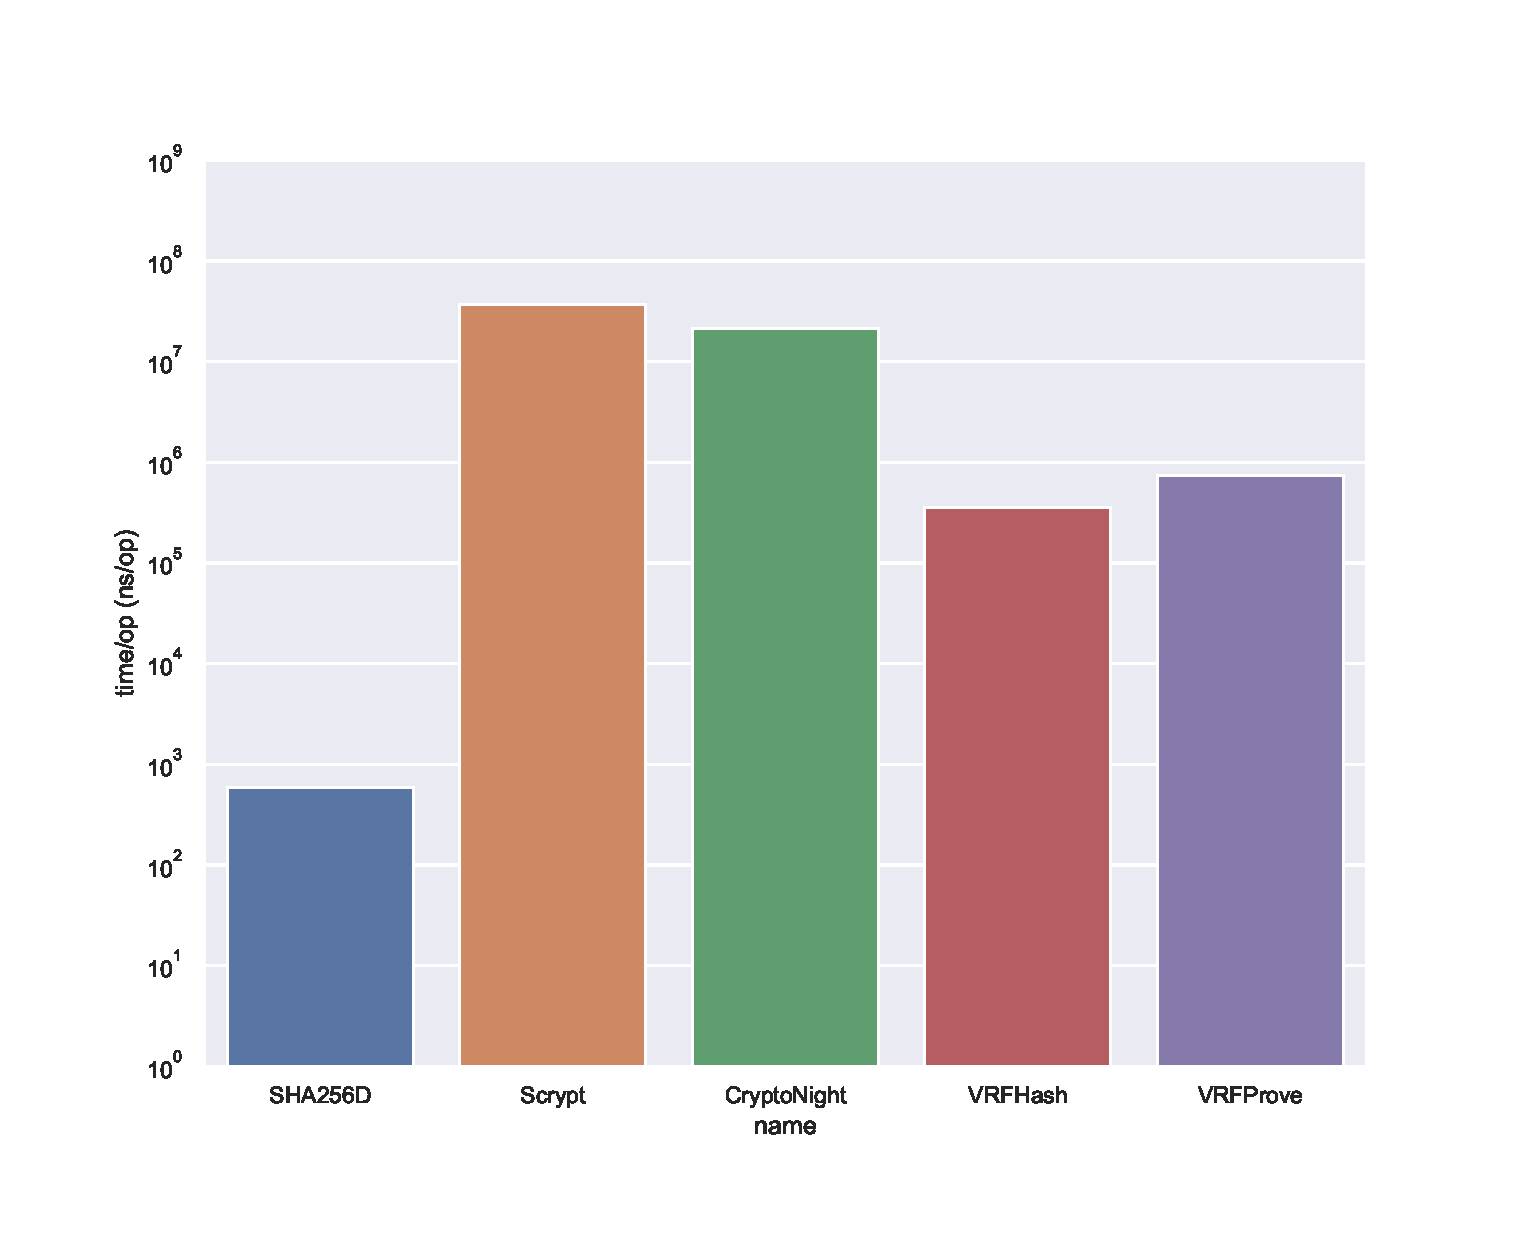
\includegraphics[width=\linewidth]{figs/runtime-comparison.eps}
    \caption{Comparing the runtime of VRF and other mining algorithms.}
    \label{fig:runtime-comparison}
\end{figure}

First, we compare the performance of VRF with other mining algorithms.
Figure~\ref{fig:runtime-comparison} shows the runtime of VRF and other algorithms.
First, SHA256D is much faster than other algorithms.
This is because SHA256D is simply executing SHA256 twice, which can be quite fast.
Second, $\mathsf{VRFVerify}$ is slightly slower than $\mathsf{VRFProve}$, and $\mathsf{VRFProve}$ is slightly slower than $\mathsf{VRFHash}$.
Last, although without optimisation, all functions of VRF are much faster than Scrypt and CryptoNight.
This means that VRF is easy to implement and introduces little overhead, so suitable for cryptocurrency mining.



\subsection{Runtime breakdown of VRF}

\begin{figure}[htp]
    \centering
    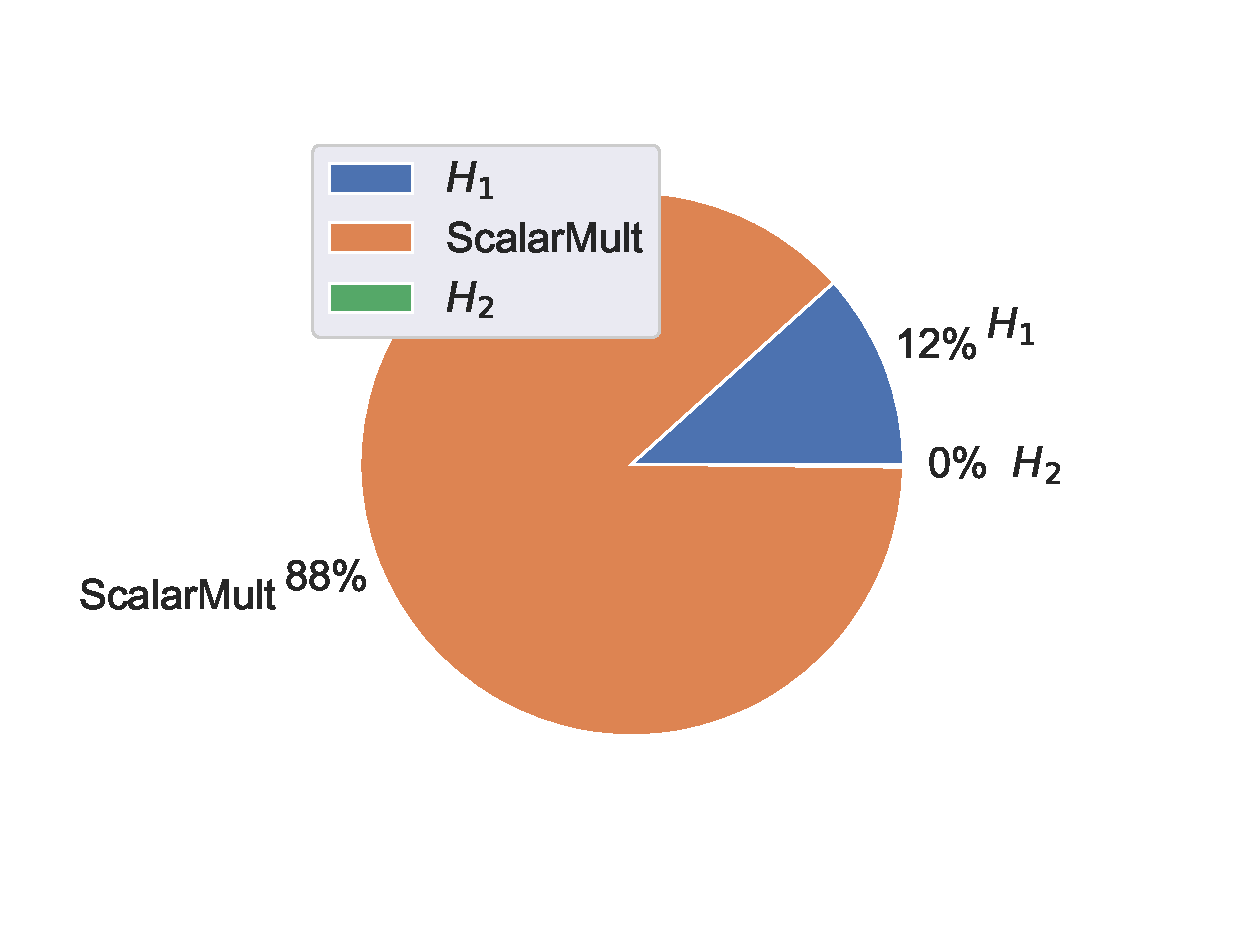
\includegraphics[width=.7\linewidth]{figs/runtime-breakdown.eps}
    \caption{Runtime breakdown of $\mathsf{VRFHash}$.}
    \label{fig:runtime-breakdown}
\end{figure}

Second, we profile $\mathsf{VRFHash}$ by evaluating its runtime of each step.
Figure~\ref{fig:runtime-breakdown} shows that, the elliptic curve scalar multiplication $\gamma \gets h^{sk}$ takes 88\% of $\mathsf{VRFHash}$'s running time.
This is as expected, as we use SHA-3 as the hash function for $H_1(\cdot)$ and $H_2(\cdot)$, and SHA-3 is designed to be fast.
Meanwhile, we calculate the elliptic curve scalar multiplication using the trivial double-and-add method without any optimisation, thus is much slower than $H_1(\cdot)$ and $H_2(\cdot)$.
Even so, $\mathsf{VRFHash}$ is still much faster than Scrypt and CryptoNight.
This further proves that VRFs introduce little overhead.
\section{Profitability of partial outsourcing}
\label{sec:partial-outsourcing}

The pool operator may still have opportunity to outsource mining partially.
$\mathsf{VRFHash}$ consists of three steps: $h \gets H_1(\alpha)$, $\gamma \gets h^{sk}$ and $\beta \gets H_2(\gamma)$.
The non-outsourceability is from the second step $\gamma = h^{sk}$, as it requires the knowledge of the pool operator's secret key $sk$.
The pool operator can outsource the first step $h = H_1(\alpha)$ by distributing different $\alpha$s to miners, and also the last step $\beta = H_2(\gamma)$ by distributing different $\gamma$s to miners.

However, such partial outsourcing is very inefficient and unprofitable compared to outsourcing in hash-based mining, due to the computing and I/O overhead.
In this section, we show that partial outsourcing in VRF-based mining is unprofitable as it's computation-intensive and I/O intensive.
We also show that making VRF fast can make VRF-based mining even more costly.

\subsection{Partial outsourcing in VRF-based mining}

\begin{figure}[htp]
    \centering
    \includegraphics[width=\linewidth]{figs/outsource-vrf.png}
    \caption{Partial outsourcing in VRF-based mining.}
    \label{fig:outsource-vrf}
\end{figure}

Figure~\ref{fig:outsource-vrf} describe the process of outsourcing $H_1(\cdot)$ and $H_2(\cdot)$.
In VRF-based mining, the second step $h^{sk}$ is non-outsourceable, but the pool operator can outsource $H_1(\cdot)$ or $H_2(\cdot)$ interactively.

To outsource $H_1(\cdot)$, the pool operator generates a search interval $[n_1, n_m]$ of nonces, then sends the interval and the block template $t$ to a miner.
After that, the miner computes $H_1(\cdot)$ with each nonce in $[n_1, n_m]$ as input, then sends back all $H_1(\cdot)$ hashes to the pool operator.
If the pool operator does not trust miners (which reflects to the real world), he will verify these $H_1(\cdot)$ hashes before the second step i.e., multiplying each hash with his secret key $sk$.

After the second step, the pool operator obtains a series of $(\gamma_1, \gamma_2, \dots, \gamma_m)$, and he can outsource $H_2(\cdot)$ as follows.
The pool operator first sends these $\gamma$s as well as the pool difficulty $PoolTarget$ to the miner.
Then, the miner calculates $H_2(\cdot)$ hashes of these $\gamma$s, compare the hashes with $PoolTarget$, and sends back $\gamma$s that satisfy the difficulty (denoted as $\Gamma$).
Similarly, the pool operator optionally verifies the correctness of each of $\Gamma$, and accumulates the mined shares to the miner's total contribution.


\subsection{The cost of verifying hashes from miners}

The first obstacle of partial outsourcing is verifying hashes from miners.
If the pool operator does not trust miners, he should verify both $H_1(\cdot)$ and $H_2(\cdot)$ hashes from miners.
Outsourcing $H_1(\cdot)$ is symmetric: The pool operator should verify all of $h_1, h_2, \dots, h_m$.
Outsourcing $H_2(\cdot)$ is asymmetric: The pool operator should only verify $\Sigma$ i.e., $\sigma$s satisfying $PoolTarget$.
This introduces significant overhead, and makes outsourcing less profitable than mining by himself for the pool operator.


\subsection{Partial outsourcing is I/O intensive}

The pool operator and miners are still possible to collaborate, as pooled mining is beneficial for them.
For the pool operator, he can earn some fees from the miners.
For the miners, they can stabilise their revenue from mining.

Even if they trust each other, partial outsourcing can still be unprofitable.
VRF-based mining can be extremely I/O intensive, while the pool operator's server suffers from limited bandwidth.
To outsource a single $H_1(\cdot)$ in VRF-based mining, the pool operator should at least receive a $H_1(\cdot)$ hash from the miner
To outsource a single $H_2(\cdot)$, the pool operator should at least send a $\sigma$ to the miner.
% hash based mining does not suffer from this problem
Hash-based mining does not suffer from this problem.
In hash-based mining, the pool operator only sends and receives constant-size data for each share.
By increasing the share difficulty, the pool operator will receive fewer shares and support more miners.

We model the maximum hashrate the pool operator can support as follows.
Consider a pool operator with bandwidth $BW$ (in Bytes/s), and the pool operator can achieve optimal bandwidth utilisation on mining.
Assume the pool operator should transfer $N$ bytes per hash.
Thus, the maximum hashrate is

$$\text{Maximum hashrate} = \frac{BW}{N}$$

Either a $H_1(\cdot)$ hash and a $\gamma$ (a point on the elliptic curve) at least takes 32 bytes.
If outsourcing both $H_1(\cdot)$ and $H_2(\cdot)$, the maximum hashrate the pool operator can support is $\text{Maximum Hashrate} = \frac{BW}{64} (h/s)$.
If outsourcing only one of them, the maximum hashrate is $\text{Maximum Hashrate} = \frac{BW}{32} (h/s)$.

\begin{figure}[htp]
    \centering
    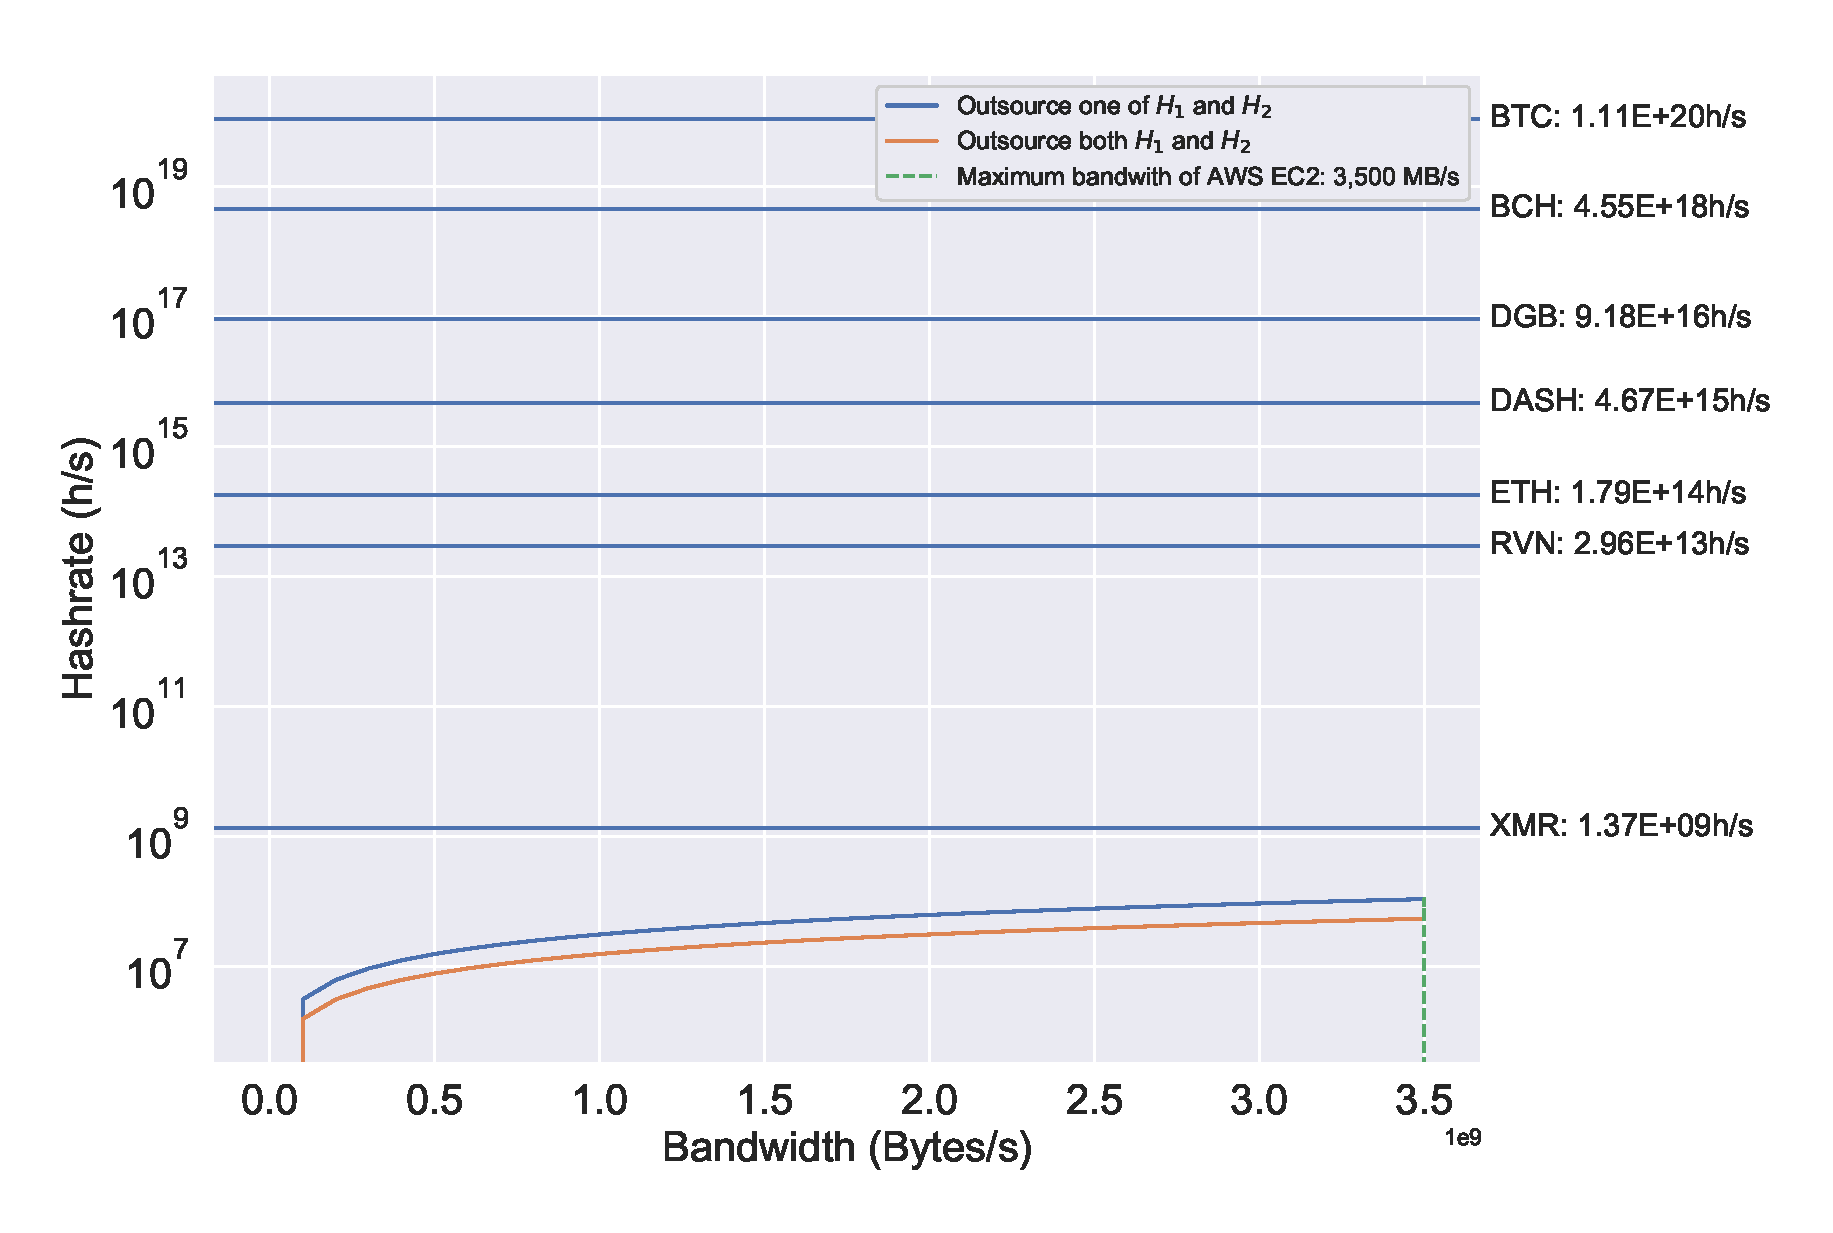
\includegraphics[width=\linewidth]{figs/max-hashrate.eps}
    \caption{Server bandwidth v.s. maximum hashrate.
    Data of server bandwidth and hashrate were fetched from \cite{aws} and \cite{coinwarz}.}
    \label{fig:max-hashrate}
\end{figure}

Figure~\ref{fig:max-hashrate} shows relationship between the pool operator's network bandwidth maximum and the maximum hashrate.
The result shows that, even a server with most bandwidth from AWS (I3EN Metal with 3,500 MB/s) can only support less than $\frac{1}{10}$ of Monero's total mining power.
Within those mainstream cryptocurrencies, Monero's hashrate is the least.
Even if the pool operator rents a cluster of I3EN Metal machines for more bandwidth, I3EN Metal is quite expensive (10.848 USD per hour), leading to high expense of maintaining a mining pool.
Therefore, partial outsourcing in VRF-based mining is costly and unrealistic.
By embedding lightweight mining algorithms in VRFs such as SHA256D, VRF-based mining can be maximally I/O-intensive.

\section{Discussions}
\label{sec:discussions}

While eliminating mining pools can improve decentralisation, it also introduces new problems.
We discuss two problems and their possible solutions, namely 1) high reward variance and 2) secret key leakage in memory.

\subsection{Weaker security guarantee of PoW-based consensus}

The reason of miners joining mining pools is that, miners may not obtain stable income via solo mining.
Miners may be discouraged to mine if their rewards are highly volatile.
With weaker incentive of mining, fewer miners will join the blockchain.
The blockchain will then attract less mining power, which weakens the security of PoW-based consensus.

This problem can be addressed by making the mining reward fine-grained.
% multi-tier
Miller et al.~\cite{miller2015nonoutsourceable} proposes the \emph{multi-tier reward scheme}.
In multi-tier reward scheme, the mining difficulty is divided into different levels, and miners can mine blocks satisfying different difficulty levels arbitrarily.
In this way, mining reward is distributed in a fine-grained way, so lowers the reward variance.
% strongchain
StrongChain~\cite{szalachowski2019strongchain} introduces the notion of Collaborative PoW, where miners are encouraged to mine blocks together and the mining reward is distributed in proportion to miners' contributions.

Another solution is to increase the rate of mining blocks.
With more blocks mined in a time unit, the mining reward can also be more stable.
For example, although of independent interest, protocols for scaling blockchains such as sharding~\cite{wang2019monoxide} and DAG~\cite{li2018scaling} can also stabilise the mining reward variance.



\subsection{Secret key leakage in memory}

VRF-mining requires the secret key, so a miner should keep his secret key in plaintext in memory \emph{all the time}.
This gives adversaries opportunity to steal the secret key from the memory.
For example, if the mining software has a bug that enables hackers to access the memory space of the mining software, then the hacker can easily steal the secret key.

% why inevitable
For VRF-based mining, keeping secret keys in memory is inevitable.
To achieve \emph{non-outsourceability}, the secret key should be combined to the mining process.
As long as mining does not stop, the secret key should be kept in plaintext in memory.
This applies to all protocols that execute frequently and require secret keys, such as TLS.

There have been several different ways to protect in-memory secret keys.
% enclave
First, the miner can isolate the scalar multiplication to a software or hardware enclave.
Note that the encalves are unnecessary to be general-purpose.
% proactive self-destroy
Second, the process of the mining software can destroy itself once detecting anomalous memory access attempts.
% isolation
Third, the miner can isolate mining from the blockchain node.
For example, it can run the mining process independently with his blockchain node process.
In this way, if an adversary compromises his node but not the operating system, the adversary still cannot read the private key in another process.
% offline
Fourth, it can run the mining process in an offline machine that can only communicate with his blockchain node.
% oram
Fifth, Oblivious RAM (ORAM) is a promising primitive to protect sensitive data in memory.
ORAM allows CPUs to access data in memory while the data in memory is encrypted and the access pattern is hidden.
% minimise
Last, the miner can use a new secret key for each block, so that leaking a secret key only affects the reward of a single block.

\section{Related work}
\label{sec:related}

To the best of our knowledge, VRF-based mining is the first construction that makes pooled mining \textit{impossible}.
We briefly review related research on preventing mining pools, and compare them with VRF-based mining.
We classify related research to two types, namely pooled-mining-unfriendly mining protocols and decentralised mining pools.

\begin{table}[t]
    \centering
    \caption{Comparison between mining protocols. NSP is short for Non-outsourceable scratch-off puzzle.}
    \begin{tabular}{ccccc}
        \hline
                                        & VRF-based mining & NSP-1 & NSP-2 & 2P-PoW \\ \hline
        Punishment                    & New reward           & New reward                                 & New reward                                 & New reward               \\
        Stealing                      & Unlinkable       & Linkable                                   & Unlinkable                                 & Unlinkable           \\
        No partial outsourcing        & \cmark           & \cmark                                     & \cmark                                     & \xmark               \\
        Support randomised signatures & \cmark           & \cmark                                     & \cmark                                     & \xmark               \\
        No complex cryptography       & \cmark           & \cmark                                     & \xmark                                     & \cmark               \\ \hline
    \end{tabular}
    \label{table:comparison-mining-protocols}
\end{table}

\begin{table}[t]
    \centering
    \caption{Comparison with decentralised mining pools.}
    \begin{tabular}{ccccc}
        \hline
                            & VRF-based mining & P2Pool & SmartPool & BetterHash \\ \hline
        Complexity       & -                & Blockchain                     & Smart contract                    & -                                      \\
        Decentralisation & Mining           & Mining                         & Mining                            & Select txs                             \\ \hline
    \end{tabular}
    \label{table:comparison-pools}
\end{table}



\subsection{Mining protocols}

There are two mining protocols aiming at discouraging or breaking mining pools: the \textit{non-outsourceable scratch-off puzzle}~\cite{miller2015nonoutsourceable} and the \textit{Two Phase Proof-of-Work} (\textit{2P-PoW})~\cite{2P-PoW}.
Table~\ref{table:comparison-mining-protocols} summarises our comparisons.

\textbf{Non-outsourceable scratch-off puzzle.}
Miller et al.~\cite{miller2015nonoutsourceable} formalises mining as \emph{scratch-off puzzles}, defines \emph{non-outsourceability}, and proposes two \emph{non-outsourceable scratch-off puzzles}.
One achieves \emph{weak non-outsourceability} --- miners can steal the mining reward, and the other achieves \emph{strong non-outsourceability} --- miners can steal the mining reward anonymously.

The weak non-outsourceable scratch-off puzzle works as follows.
First, the miner randomly generates a Merkle tree.
Second, the miner randomly chooses a nonce, samples some leaves of the Merkle tree according to the nonce, and hashes their Merkle proofs together to a single hash.
If this hash meets the difficulty requirement, then the nonce is valid.
Last, the miner binds the valid nonce and his block template together to a valid block.

In order to outsource the mining process, the mining pool should distribute the search space of nonces to miners.
% how to steal
A miner can steal the mining reward by binding valid nonces it finds with his own block template.
% why weak
However, this stealing process is not anonymous.
Unlike existing PoW-based consensus where miners can choose both nonces and block templates, the weak non-outsourceable scratch-off puzzle only allows miners to choose nonces, so all miners share the same search space of nonces.
Thus, the pool operator can link the nonce in the stolen block with the miner who is assigned with the search space covering this nonce.
To achieve \emph{strong non-outsourceability}, the strong non-outsourceable scratch-off puzzle replaces the plaintext nonce in the block with a Zero Knowledge Proof proving the statement ``I know a valid nonce''.

As discussed in \S\ref{sec:non_outsourceability}, while being simpler and more efficient than non-outsourceable scratch-off puzzle, our VRF-based mining achieves \emph{strong non-outsourceability}.

\textbf{2P-PoW.}
Eyal and Sirer proposes 2P-PoW~\cite{2P-PoW}, a mining protocol that discourages pooled mining.
In 2P-PoW, mining consists of two phases, and each phase has a difficulty parameter.
A miner should find a nonce that makes the block to pass two phases: 1) the SHA256D hash of the block meets the first difficulty, 2) the SHA256 hash of the signature of the block meets the second difficulty.
As the second requirement requires the private key, pool operators cannot outsource the second phase.

% first phase outsourceable
Compared to VRF-based mining that makes pooled mining impossible, 2P-PoW is partially outsourceable by outsourcing the first phase.
% det sig
In addition, 2P-PoW requires the digital signature algorithm to be deterministic, while commonly used digital signatures such as ECDSA rely on randomisation.
If the signature is randomised, the pool operator can make use of all nonces from miners that meet the first phase but fail the second phase.
Given a nonce meeting the first difficulty, the pool operator repetitively generates signatures to meet the second requirement.
% diff
Moreover, how to adjust two difficulties still remains unknown and requires some simulations.




\subsection{Decentralised mining pools}


% ref: https://www.alexeizamyatin.me/files/Decentralized_Mining-Security_and_Attacks.pdf

Decentralised mining pool is a type of mining pools that work in a decentralised way: miners mine in the name of themselves and share reward in a fine-grained way.
In this way, miners are rewarded stably while mining power is not controlled by pool operators.
Table~\ref{table:comparison-pools} summarises the comparison between VRF-based mining with decentralised mining pools.


\textbf{P2Pool}~\cite{voight2011p2pool} is a decentralised mining pool for Bitcoin.
% how p2pool works
Instead of using a centralised server, P2Pool uses a blockchain called \emph{share-chain} to receive shares from miners.
All miners in P2Pool participate in the PoW-based consensus of share-chain.
Once a miner finds a share on Bitcoin, it appends a block to the share-chain.
The block consists of the share and a coinbase transaction that rewards miners in proportion to their shares.
Once a miner mines a block that also satisfies Bitcoin's difficulty, it submits this block to the Bitcoin blockchain, and and miners are rewarded according to the coinbase transaction.
% challenges
P2Pool suffers from several limitations.
First, handling the difficulty of mining shares is hard.
If the difficulty is high, miners' reward will still be volatile.
If the difficulty is low, there will be numerous low-difficulty shares, which introduces huge overhead on broadcasting and receiving shares.
Second, shares on share-chain are much more frequent than blocks on Bitcoin blockchain, and the share-chain suffers from high orphan rate.
Last, existing research shows that P2Pool is vulnerable to temporary dishonest majority~\cite{decentralised-mining-pool-security}.

\textbf{SmartPool}~\cite{luu2017smartpool} is another decentralised mining pool.
Instead of using a blockchain, SmartPool employs smart contracts to track shares from miners.
% con 1: smart contract
This implies that SmartPool cannot work on blockchains without smart contracts.
% con 2: network delay
In addition, as blockchains achieve limited throughput, blockchains can only handle a limited number of shares for each time unit.
In this way, distributing mining reward may also be delayed, especially when a large number of miners participate in the SmartPool.
% con 3: compute and storage overhead
Moreover, as the SmartPool smart contract should verify the validity of blocks, miners should submit the entire block --- including transactions --- to the SmartPool.
Verifying blocks introduces non-negligible computing overhead and transaction fee, and storing blocks in smart contracts also introduces non-negligible overhead on storage.



\textbf{BetterHash}~\cite{draft-bip-BetterHash} is another decentralised mining protocol, which has been integrated into \emph{Stratum V2}~\cite{stratum-v2}, the next generation of the \textit{Stratum}~\cite{stratum} pooled mining protocol.
In \textit{BetterHash}, the block operator allows miners to choose transactions and construct blocks in his name, rather than constructing block templates by himself.
Thus, \textit{BetterHash} only contributes to the decentralisation of constructing blocks, but does not improve the decentralisation of mining power.
\section{Conclusion and future work}
\label{sec:conclusion}

In this paper, we propose VRF-based mining, that can make pooled mining in Proof-of-work-based consensus impossible.
VRF-based mining is simple and intuitive: miners produce digests of blocks using VRFs rather than hash functions, so that a pool operator should reveal his secret key to outsource the mining process to other miners.
We informally prove that VRF-based mining achieves the strongest notion of \emph{non-outsourceability}.
In addition, we discuss considerations of instantiating VRF-based mining.
Moreover, we experimentally proves that VRF-based mining is simple to implement and introduces negligible overhead.

\bibliographystyle{ieeetran}
\bibliography{refs}

\appendix
\section{Standardised construction of VRF}

Let $G$ be a cyclic group of prime order $q$ with generator $g$. Assume $E = G$
Let $H_1(\cdot)$ be a hash function mapping an arbitrary-length string into an element in $G$.
Let $H_2(\cdot)$ be a hash function mapping an element in $G$ into a fixed-length string.
Let $H_3(\cdot)$ be a hash function mapping an arbitrary-length string into a fixed-length string.

$(sk, pk) \leftarrow VRFKeyGen(1^{\lambda})$
\begin{enumerate}
    \item $sk$ is chosen uniformly and randomly from $\interval{0}{q-1}$
    \item $pk = g^{sk}$
\end{enumerate}

$h \leftarrow VRFHash(sk, \alpha)$
\begin{enumerate}
    \item $h = H_{1}(\alpha)$
    \item $\gamma = h^{sk}$
    \item $\beta = H_{2}(\gamma)$
\end{enumerate}

$\pi \leftarrow VRFProve(sk, \alpha)$
\begin{enumerate}
    \item $h = H_{1}(\alpha)$
    \item $\gamma = h^{sk}$
    \item choose a random $k \in \interval{0}{q-1}$
    \item $c = H_{3}(g, h, pk, h^{sk}, g^{k}, h^{k})$
    \item $s = k - c \cdot sk \pmod{q}$
    \item $\pi = (\gamma, c, s)$
\end{enumerate}

$\{0, 1\} \leftarrow VRFVerify(pk, \alpha, \beta, \pi)$
\begin{enumerate}
    \item $u = pk^{c} \cdot g^{s}$
    \item $h = H_{1}(\alpha)$
    \item check if $\gamma \in G$
    \item $v = \gamma^{c} \cdot h^{s}$
    \item check if $c \stackrel{?}{=} H_{3}(g, h, pk, \gamma, u, v)$
\end{enumerate}


\end{document}